\chapter{提案手法}
関連研究の章ではニューラルネットワークや決定木が内包する説明性の欠如という問題点と説明を加える既存手法の持つ課題について述べた。
本論文ではそれらを踏まえた
\begin{itemize}
	\item 本来ゲームに存在する時系列の要素を含む
	\item 評価基準が勝敗に直結する
    \item 人間のドメイン知識に依存しない
\end{itemize}
説明手法を提案する。
本手法はある状態$s$においてAIが予想する未来図$o(s)$とそこに至るまでの道筋を取り出すことで$s$におけるAIの判断$a$
の意図を可視化することを目標とする。


\section{実装}
本手法はAlphaZeroシステムのニューラルネットワークと木探索部分のうち、主に木探索の部分を対象に適用される。
本手法では決定木の判断を説明する際に最も有用な部分を決定木から抽出することを主な目的としており、アルゴリズムは決定木構造を持つ多くのシステムに応用可能である。
アルゴリズムの主な流れは以下の通りである。
1:説明を付与する状態$s_{start}$を選択する。このとき$s_{start}$に対するモデルの方策$P(s_{start})$が推奨する行動$a_m$を取り出す。
このとき注目している状態$s_{now}, a_{now}$はそれぞれ
\begin{equation}
	{s_{now}=s_{start},}
	{a_{now}=a_m}
\end{equation}
とする。
2:以下の流れを$l$ステップ分繰り返す
決定木中の注目しているード$s_{now}$における方策$P(s_{now})$中の値にして上位$k$個分の行動${a_0, a_1, ..., a_{k-1}}(a_iはk+1番目に有望な行動とする)$を取り出す。
${s_{next_0}, s_{next_1}, ..., s_{next_{k-1}}}(s_{next_i}=T(s_{now}, a_i), Tは遷移関数)$の各ノードに対してstep2
の操作を繰り返す。プログラム上は探索の開始地点$s_{start}$からstep2中にたどり着く各ノード$s_{middle}$までの軌道$\rm{{traj}_{s_middle}}(=[{a'}_{t_0}, {a'}_{t_1}, ..., {a'}_{t_{l-1}}]、 t_iはi番目のステップを表す)$を記録しておく。

3:集めた$k$の$l$乗枚の盤面ノード${{s}'_{0}, {s'}_{1}, ..., {s'}_{k^l-1}}$のそれぞれ${s'}_{i}(i=0, 1, ..., k^l-1)$対して以下の操作を再帰的に繰り返す。
${s'}_{i}$における方策$P({s'}_{i})$中の最も有望な行動$a_{promising}$と${s'}_{next_i}=T({s'}_i, a_{promising})$を記録する。
そのようにして記録した${{s'}_{next_0}, {s'}_{next_1}, ..., {s'}_{next_{k^l-1}}}$のそれぞれ${s'}_{next_j}(j=0の, 1, ..., k^l-1)$にも同様の動作を盤面ノードが決定木の端に辿り着くまで行う。
step2と同様に探索の開始地点$s_{start}$からstep3中にたどり着く各ノード$s_{middle}$への軌道$\rm{{traj}_{s_middle}}(=[{a'}_{t_0}, {a'}_{t_1}, ..., {a'}_{t_{l-1}}, {a'}_{t_l}, {a'}_{t_{l+1}}, ..., {a'}_{t_p}]、 t_iはi番目のステップを表す)$を記録しておく。
4:step3によってたどり着いた$k^l$個のノードによる集合$S={s_{edge_0}, s_{edge_1}, ..., s_{edge_{k^l-1}}}$をなんらかの共通項$c$によっていくつかの副集合${S_0, S_1, ..., S_q}$に分ける。
5:共通項で括られた各集合${S_0, S_1, ..., S_q}$のうち、最も要素数が多いもの$S_{max}$中の各要素${s_{e_0}, s_{e_1}, ...,  s_{e_u}}$と各要素に対応する軌道${\rm{{traj}_{s_{e_0}}}, \rm{{traj}_{s_{e_1}}}, ...,  \rm{{traj}_{s_{e_u}}}}$を抽出する。
このアルゴリズムを要約するとある局面$s$と行動$a$の組み合わせから最も辿り着きやすい結末$O(s, a)$を抽出し、$O(s, a)$に至るまでの複数の道筋を抽出すると表現できる。
調査を行う者が複数の軌道を観察できることで、
共通する傾向や法則性を見出せるというメリットが存在する。これは最も可能性が高い一つの分岐を示す、といったような情報が単一である手法には不可能である。
\begin{figure}[t]
	\centering
	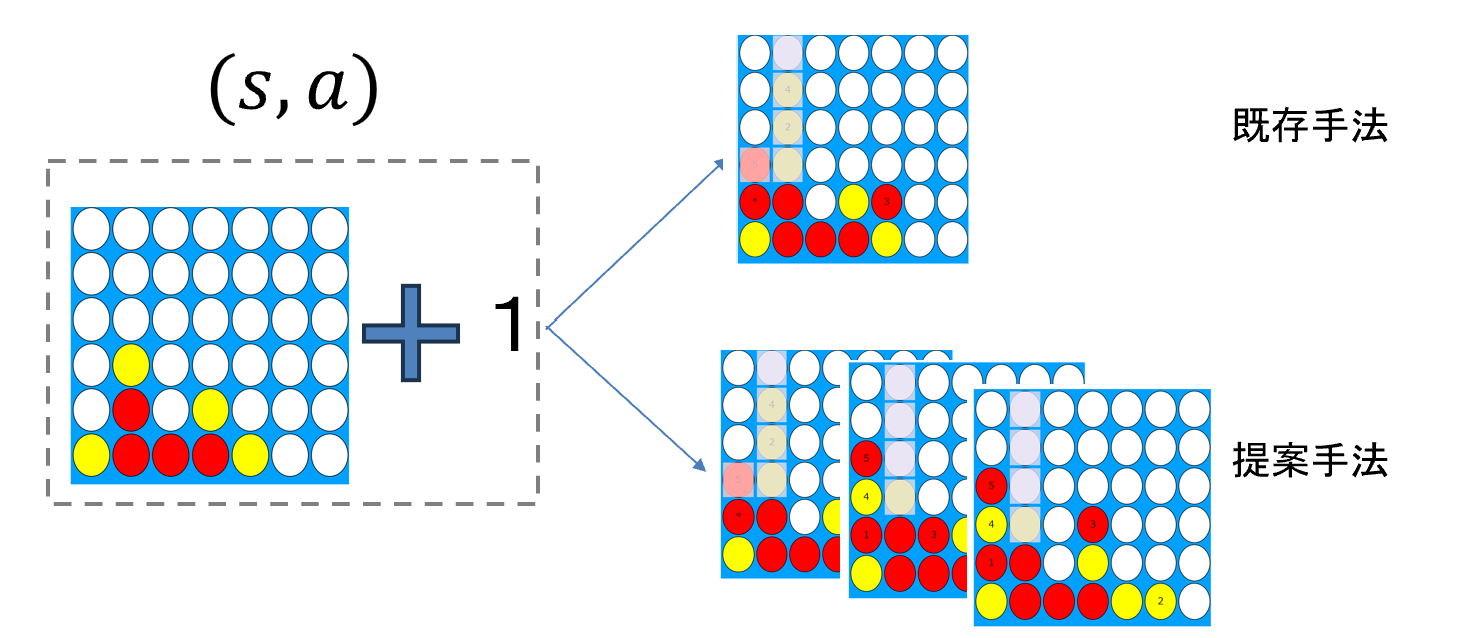
\includegraphics[width=\linewidth]{./figure/merit.png}
	\caption{提案手法のイメージ}
	\label{fig:merit}
\end{figure}
\begin{algorithm}
    \caption{提案手法のアルゴリズム}
    \begin{algorithmic}[1]
        \State Select initial state $s_{start}$ with policy $P(s_{start})$ recommending action $a_m$
        \State Set $s_{now} = s_{start}$ and $a_{now} = a_m$
        \For {$l$ steps}
            \State Retrieve top $k$ actions ${a_0, a_1, ..., a_{k-1}}$ from policy $P(s_{now})$ at node $s_{now}$
            \For {each action $a_i$}
                \State Calculate $s_{next_i} = T(s_{now}, a_i)$ using transition function $T$
                \State Apply steps 2 and 3 to $s_{next_i}$ recursively
            \EndFor
            \State Record trajectory ${\rm{traj}_{s_{now}}}$ from $s_{start}$ to each visited node $s_{middle}$
        \EndFor
        \State Apply step 4 to obtain sets $S = \{s_{edge_0}, s_{edge_1}, ..., s_{edge_{k^l-1}}\}$
        \State Apply step 5 to find the largest subset $S_{max}$ and extract trajectories for each element
    \end{algorithmic}
\end{algorithm}


次章で示すようにconnect4タスクにおいて収集される軌道の集合においては末端部分のいくつかの選択が共通している傾向が確認された。
そのため状態と行動の組$(s, a)$から$O(s, a)$という結果を予測する過程で$O(s, a)$から末尾の数手を取り除いた版面$d$にたどり着く傾向の発見などの知識獲得が記載される。
\section{importance}
前章で述べたように、エピソード中の各状態$s$の重要度$I(s)$の定義を以下のように定めた。
\begin{equation}
	{I(s)=V[Q'] (Q'=[\rm{max}Q(s, a), \rm{secondMax}Q(s, a), ..., \rm{thirdQuantile}Q(s, a)])}
\end{equation}
つまり、現在の状態$s$に対する行動の集合$A(={a_0, a_1, ..., a_N})$とした際の行動価値関数の集合${Q(s, a_0), Q(s, a_1), ..., Q(s, a_N)}$のうち大きさが上位75
\%の成分で構成される集合の分散として重要度$I(s)$を定義する。
これは次の一手で辿り着きうる収益の予想の揺らぎの幅を意味しており、先述した盤面の対称性や悪い選択肢の影響が大きくなる可能性の軽減が期待できる。

